\chapter{Memory management in NekPy}

One of the biggest technical challenges of the NekPy project was to ensure the appropriate 
memory management between Python and C++. The computations carried out in \nek{} are 
usually highly demanding on the machines they are run on, therefore any unnecessary data 
duplication or memory leaks would be detrimental to software performance.

This section outlines the basics of memory management in C++ and Python as well as the 
solutions devised to effectively use the resources when passing data between the different 
layers of the bindings.

\section{Memory management in C++ and Python}

\subsection{C++}

In C++ the memory used by the application is divided into five containers \cite{C++Memory}:
\begin{itemize}
    \item text segment -- containing the set of instructions for the program to execute;
    \item data segment -- containing static and global variables initialised with values, 
    e.g. \texttt{float pi = 3.14;} -- the size of the data segment is pre-determined at 
    the time of the compilation of the program and depends on the size of the variables 
    in the source code;
    \item bss (block started by symbol) segment -- containing static and global variables 
    not explicitly initialised with any value, e.g. \texttt{int n;} -- the size of the 
    data segment is pre-determined at the time of the compilation of the program and 
    depends on the size of the variables in the source code;
    \item stack -- a LIFO (last in, first out) structure containing the function calls 
    and variables intialised in the functions -- the size of the stack is pre-determined 
    at the time of compilation of the program and depends on the operating system and 
    development environment;
    \item heap -- containing all dynamically allocated memory (e.g. using instruction 
    \texttt{new} in C++).
\end{itemize}

The access to data on the heap is maintained by pointers which store the memory address of 
said data. If the pointer ceases to exist (e.g. because the function which contained it 
finished running and hence was taken off the stack) the programmer has no way of referencing 
the data on the heap again. The unused, inaccessible data will stay in the memory, consuming 
valuable resources if not properly deallocated using \texttt{delete} instruction. Issues may 
arise if the same memory address is held by two different pointers -- the deallocation of 
memory can render one of the pointers empty and possibly lead to errors.

In order to facilitate memory management, C++11 standard introduced shared pointers 
(\texttt{shared\_ptr}) \cite{C++SharedPtr}. Shared pointers maintain a reference counter 
which is increased when another shared pointer refers to the same memory address. The memory 
will only be deallocated when all shared pointers referencing the memory are destroyed, as shown 
in Figure \ref{fig:shared_ptr}.

\begin{figure}[h!]
    \centering
    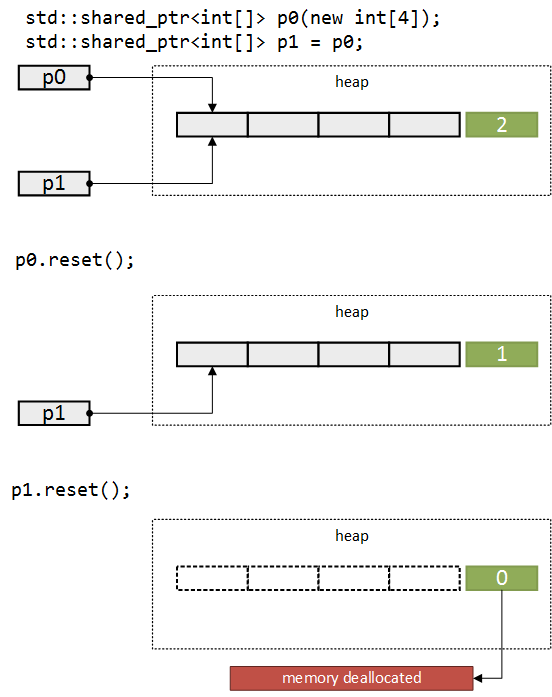
\includegraphics[width=0.6\textwidth]{img/shared_ptr}
    \caption{Memory management with C++11 \texttt{shared\_ptr}. The two declared shared pointers 
    reference an array of 4 integers. Reference counter shown in green.}
    \label{fig:shared_ptr}
\end{figure}

\subsubsection{Python}

Python manages memory though a private heap containing all Python objects \cite{PythonMemory}. 
An internal memory manager is used to ensure the memory is properly allocated and dealocated 
while the script runs. In contrast to C++, Python Memory Manager tries to optimise the memory 
usage as much as possible. For example, the same object reference is allocated to a new variable 
if the object already exists in memory. Another important feature of Python Memory Manager is 
the use of garbage collector based on reference counting. When the object is no longer referenced 
by any variable the reference counter is set to zero which triggers the garbage collector to free 
the memory. A disadvantage of this solution is slower execution time, since the garbage collector 
routines have to be called frequently. Features of Python Memory Manager are schematically shown 
in Figure \ref{fig:python_gc}

\begin{figure}[h!]
    \centering
    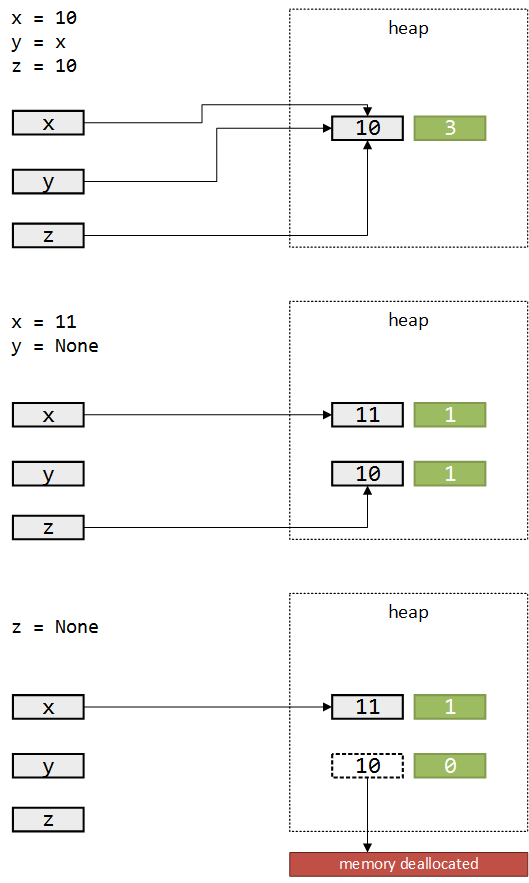
\includegraphics[width=0.6\textwidth]{img/python_gc}
    \caption{Memory management in Python. Memory is optimised as much as possible and garbage 
    collector deallocates the memory if the reference counter (shown in green) reaches 0.}
    \label{fig:python_gc}
\end{figure}

It is unusual for the Python programmer to manually modify the way Python uses memory resources 
-- however it is sometimes necessary, as is the case with this project. In particular, 
Python enables the programmer to increase or decrease the reference counter of the object 
using \texttt{Py\_XINCREF} and \texttt{Py\_XDECREF} respectively \cite{PythonManualMemory}.

\section{Passing C++ arrays to Python}
The file implementing the below procedure: \texttt{LibUtilities\/Python\/LinearAlgebra\/NekMatrix.cpp}.

In many situations arrays created by Nektar++ (usually a \texttt{shared\_ptr} of 
\texttt{NekMatrix<D, StandardMatrixTag>} type) in C++ need to be passed to Python - 
for instance, when preforming differentiation using e.g. Gauss quadrature rules a 
differentiation matrix must be obtained. In order to keep the program memory efficient 
the data should not be copied into a NumPy array but rather be referenced by the Python 
interface. This, however, complicates the issue of memory management.

Consider a situation, where C++ program no longer needs to work with the generated array 
and the memory dedicated to it is deallocated. Meanwhile, Python interface might still require 
the data contained within the array, only to be faced with an error as the data no longer 
exists in memory. To prevent such situations a solution employing reference counting must be used.

\subsubsection{Converter method}

Boost.Python provides the methods to do both convert a C++ type element to one recognised by 
Python as well as to maintain appropriate reference counting. Listing \ref{lst:c_to_python} 
shows an abridged version of the converter method (for Python 2 only) with comments on 
individual parameters. The object requiring conversion is a \texttt{shared\_ptr} of 
\texttt{NekMatrix<D, StandardMatrixTag>} type (named \texttt{mat}).

\begin{lstlisting}[caption={Converter method for converting the C++ arrays into Python NumPy arrays.}, label={lst:c_to_python}, language=C++]
#include <LibUtilities/LinearAlgebra/NekMatrix.hpp>
#include <LibUtilities/LinearAlgebra/MatrixStorageType.h>
#include <NekPyConfig.hpp>

using namespace Nektar;
using namespace Nektar::LibUtilities;

template<typename T, typename F>
void NekMatrixCapsuleDestructor(void *ptr) // destructor for the shared_ptr to data
{
    std::shared_ptr<NekMatrix<T, F>> *mat =
        (std::shared_ptr<NekMatrix<T, F>> *)ptr;
    delete mat;
}

template<typename T>
struct NekMatrixToPython
{
    static PyObject *convert(
        std::shared_ptr<NekMatrix<T, StandardMatrixTag>> const &mat)
    {
    py::object capsule(
            py::handle<>(PyCObject_FromVoidPtr(
                             new std::shared_ptr<NekMatrix<T, StandardMatrixTag>>(mat), // new shared_ptr to the data
                             NekMatrixCapsuleDestructor<T, StandardMatrixTag>))); // destructor method
                             
    int nRows = mat->GetRows(), nCols = mat->GetColumns();
    
    return py::incref( // increments Python reference counter
            np::from_data(
                mat->GetRawPtr(), // pointer to data
                np::dtype::get_builtin<T>(), // data type
                py::make_tuple(nRows, nCols), // shape of the array
                py::make_tuple(sizeof(T), nRows * sizeof(T)), // stride of the array
                capsule).ptr()); // capsule - contains the object owning the data (preventing it from being prematurely deallocated)
\end{lstlisting}

First, a new Python object is created, holding a shared pointer (\texttt{PyCObject\_FromVoidPtr}) 
to the array held in memory, increasing its reference counter and preventing it from being 
prematurely deallocated, as shown in Figure \ref{fig:c_to_python}, as well as destructor which 
contains instructions on what is to be done when the object is no longer needed (in this case, 
the \texttt{shared\_ptr} is to be deleted). It is worth noting that the steps (c) and (d) can 
be reversed and the \texttt{shared\_ptr} created by the Python binding can be removed first. 
In this case the memory will be deallocated only when the \texttt{shared\_ptr} created by C++ 
is also removed.

\begin{figure}[h!]
    \centering
    \begin{subfigure}{0.6\textwidth}
        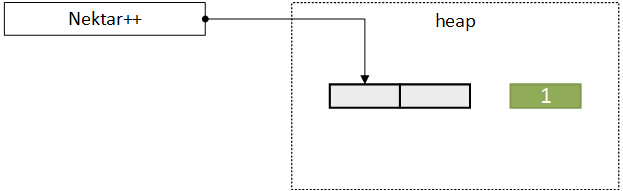
\includegraphics[width=0.99\textwidth]{c_to_python_a}
        \caption{Nektar++ creates a data array referenced by a \texttt{shared\_ptr}}
        \label{fig:c_to_python_a}
    \end{subfigure}
    \begin{subfigure}{0.6\textwidth}
        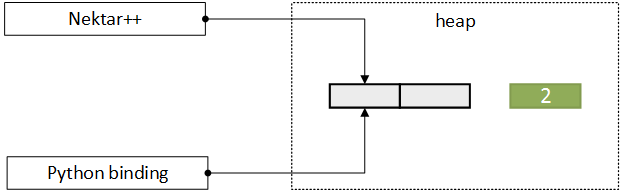
\includegraphics[width=0.99\textwidth]{c_to_python_b}
        \caption{Array is passed to Python binding which creates a new \texttt{shared\_ptr} 
        to the data}
        \label{fig:c_to_python_b}
    \end{subfigure}
    \begin{subfigure}{0.6\textwidth}
        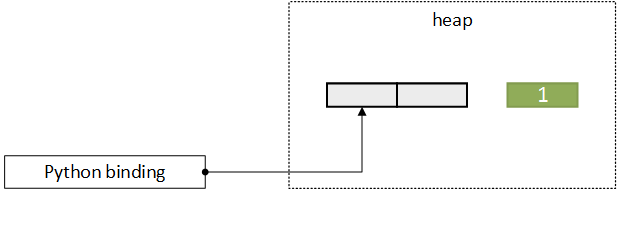
\includegraphics[width=0.99\textwidth]{c_to_python_c}
        \caption{Nektar++ no longer needs the data - its \texttt{shared\_ptr} is removed but 
        the memory is not deallocated}
        \label{fig:c_to_python_c}
    \end{subfigure}
    \begin{subfigure}{0.6\textwidth}
        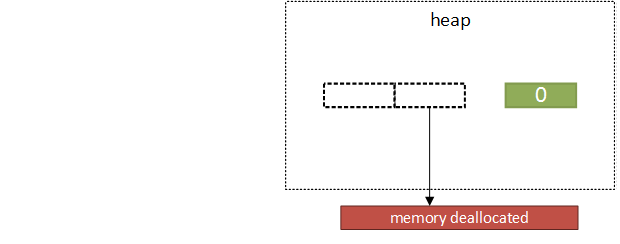
\includegraphics[width=0.99\textwidth]{c_to_python_d}
        \caption{When the data is no longer needed in the Python interface the destructor is 
        called and \texttt{shared\_ptr} is removed.}
        \label{fig:c_to_python_d}
    \end{subfigure}
    \caption{Memory management of data created in C++ using \texttt{shared\_ptr} and passed 
    to Python. Reference counter shown in green.}
    \label{fig:c_to_python}
\end{figure}

Then, a Boost.Python handle is created around the object, allowing Boost.Python to manage references 
correctly. Finally, a Boost.Python object named \texttt{capsule} is created from the handle.

The converter method returns a NumPy array -- this was chosen as it is a well-known datatype used 
in Python's popular \texttt{numpy} package. Additionally, Boost.Python allows the programmer to 
create a NumPy array from a generic C++ data container and to specify the owner of said container 
using the \texttt{np::from\_data} method. 

Care had to be taken to ensure that the array is presented in the correct order, especially as 
Nektar++ stores data in column major order whereas NumPy arrays are traditionally row major. 
The stride of the array has to be passed into the \texttt{np::from\_data} in a form of 
\texttt{(a, b)} tuple, where \texttt{a} is the number of bytes needed to skip to get to the 
same position in the next row and \texttt{b} is the number of bytes needed to skip to get to the 
same position in the next column. Hence, the tuple passed was \texttt{(sizeof(T), nRows * sizeof(T))}, 
where \texttt{T} is the datatype of the array.

In order to stop Python from immediately destroying the resulting NumPy array, its reference counter 
is manually increased before the array is passed on to Boost.Python and eventually returned to the user.

\subsubsection{Testing}

The process outlined above requires little manual intervention from the programmer. There are no almost 
no explicit calls to Python C API (aside from creating a \texttt{PyObject} -- \texttt{PyCObject\_FromVoidPtr}) 
as all operations are carried out by Boost.Python. Therefore, the testing focused mostly on correctness 
of returned data, in particular the order of the array.

To this end, the \emph{Differentiation} tutorials were used as tests. In order to correctly run the 
tutorials the Python wrapper needs to retrieve the differentiation matrix which, as mentioned before, 
has to be converted to a datatype Python recognises. The test runs the differentiation tutorials and 
compares the final result to the fixed expected value. The test is automatically run as a part of 
\texttt{ctest} command if both the Python wrapper and the tutorials have been built.

\subsection{Passing Python data to C++} 
The files implementing the below procedure are: \texttt{LibUtilities/Python/BasicUtils/SharedArray.cpp} and \texttt{LibUtilities/BasicUtils/SharedArray.hpp}

Conversely, a similar problem exists when data is created in Python and has to be passed to 
the C++ program. In this case, as the data is managed by Python, the main reference counter 
should be maintained by the Python object and incremented or decremented as appropriate 
using \texttt{Py\_XINCREF} and \texttt{Py\_XDECREF} methods respectively.

When the array is no longer needed by the C++ program the reference counter on the Python 
side should be decremented in order for Python garbage collection to work appropriately 
-- however this should only happen when the array was created by Python in the first place. 

\subsubsection{Modifications to \texttt{Array<OneD, const DataType>} class template}

In order to perform the operations described above, the C++ array structure should contain 
information on whether or not it was created from data managed by Python. To this end, 
two new attributes were added to C++ \texttt{Array<OneD, const DataType>} class template:

\begin{itemize}
    \item \texttt{m\_memory\_pointer} - holding the pointer to the 
        \texttt{PyObject} containing the data,
    \item \texttt{m\_python\_decrement} - holding the pointer to the 
        callback function decrementing the reference counter of the \texttt{PyObject}.
\end{itemize}

If the two new attributes are not set to \texttt{nullptr} the array has been constructed 
throught the Python to C++ converter. The already existing \texttt{m\_count} attribute 
was retained in order to keep track of how many C++ references to the array there are.

Adding new attributes to the arrays might cause a significantly increased memory usage. 
Therefore a preprocessor directive has been added to only include the additional arguments 
if \texttt{NekPy} had been built (using the option \texttt{NEKTAR\_BUILD\_PYTHON}).

A new constructor has been added to the class template, as seen in Listing \ref{lst:new_const}. 
\texttt{m\_memory\_pointer} and \texttt{m\_python\_decrement} have been set to 
\texttt{nullptr} in the pre-existing constructors. A similar constructor was added for 
\texttt{const} arrays to ensure that these can also be passed between the languages. Note that 
no calls to Nektar++ array initialisation policies are made in this constructor, unlike in 
the pre-existing ones, as there is no need for the new array to copy the data.

\begin{lstlisting}[caption={New constructor for initialising arrays created through the Python to C++ converter method.}, label={lst:new_const}, language=C++]
Array(unsigned int dim1Size, DataType* data, void* memory_pointer, void (*python_decrement)(void *)) :
                m_size( dim1Size ),
                m_capacity( dim1Size ),
                m_data( data ),
                m_count( nullptr ),
                m_offset( 0 ),
                m_memory_pointer( memory_pointer ),
                m_python_decrement( python_decrement )
            {
                m_count = new unsigned int(); 
                *m_count = 1;
            }
\end{lstlisting}

Changes have also been made to the destructor, as shown in Listing \ref{lst:destructor}, 
in order to ensure that if the data was initially created in Python the callback function 
would decrement the reference counter of the NekPy array object. The detailed procedure 
for deleting arrays is described further in this section.

\begin{lstlisting}[caption={The modified destructor for C++ arrays.}, label={lst:destructor}, language=C++]
~~Array()
            {
                if( m_count == nullptr )
                {
                    return;
                }

                *m_count -= 1;
                if( *m_count == 0 )
                {
                    #ifdef WITH_PYTHON
                    if (m_memory_pointer == nullptr)
                    {
                        ArrayDestructionPolicy<DataType>::Destroy( m_data, m_capacity );
                        MemoryManager<DataType>::RawDeallocate( m_data, m_capacity );
                    }
                    else
                    {
                        m_python_decrement(m_data);
                    }
                    #else
                    ArrayDestructionPolicy<DataType>::Destroy( m_data, m_capacity );
                    MemoryManager<DataType>::RawDeallocate( m_data, m_capacity );
                    #endif
                  
                    delete m_count; // Clean up the memory used for the reference count.
                }
            }
\end{lstlisting}

\subsubsection{Creation of new arrays}

The following algorithm has been proposed to create new arrays in Python and allow the 
C++ code to access their contents:

\begin{enumerate}
    \item A new NumPy array object is created in Python.
    \item The NumPy array object is passed as an argument to a C++ method available in 
        the Python wrapper.
    \item The converter method is called to convert a Python NumPy array into C++ 
        \texttt{Array<OneD, const DataType>} object.
    \item The converter creates a new \texttt{Array<OneD, const DataType>} object with the 
        following attribute values:
    \begin{itemize}
        \item \texttt{m\_data} points to the data contained by the NumPy array,
        \item \texttt{m\_memory\_pointer} points to the NumPy array object,
        \item \texttt{m\_python\_decrement} points to the function decrementing the 
            reference counter of the \texttt{PyObject},
        \item \texttt{m\_count} is equal to 1.
    \end{itemize}
    \item The Python reference counter of the NumPy array object is increased.
    \item If any new references to the array are created in C++ the \texttt{m\_count} 
        attribute is increased accordingly. Likewise, if new references to NumPy array 
        object are made in Python the reference counter increases.
\end{enumerate}

The process is schematically shown in Figure \ref{fig:array_creation_deletion_a} 
and \ref{fig:array_creation_deletion_b}.

\subsubsection{Array deletion}

The array deletion process relies on decrementing two reference counters: one 
on the Python side of the program (Python reference counter) and the other one 
on C++ side of the program. The former registers how many Python references to 
the data there are and if there is a C++ reference to the array. The latter 
(represented by \texttt{m\_count} attribute) counts only the number of references 
on the C++ side and as soon as it reaches zero the callback function is triggered to 
decrement the Python reference counter so that registers that the data is no longer 
referred to in C++. Figure \ref{fig:array_deletion} presents the overview of the 
procedure used to delete the data.

In short, the fact that C++ uses the array is represented to Python as just an 
increment to the object reference counter. Even if the Python object goes out 
of scope or is explicitly deleted, the reference counter will always be non-zero 
until the callback function to decrement it is executed, as shown in Figure 
\ref{fig:array_creation_deletion_c}. Similarly, if the C++ array is deleted first, 
the Python object will still exist as the reference counter will be non-zero 
(see Figure \ref{fig:array_creation_deletion_d}).

\subsubsection{Converter method}

As with conversion from C++ to Python, a converter method was registered 
to make Ptyhon NumPy arrays available in C++ with Boost.Python. 
Listing \ref{lst:python_to_c} shows the converter methods with comments on its contents.

In essence, Boost.Python provides the used with a memory segment (all expressions 
containing \linebreak \texttt{rvalue\_from\_python} are to do with doing that). The 
data has to be extracted from PyObject in order to be presented in a format C++ knows 
how to read -- the \texttt{get\_data} method allows the programmer to do it for 
NumPy arrays. Finally, care must be taken to manage memory correctly, thus the 
use of borrowed references when creating Boost.Python object and the incrementation 
of PyObject reference counter at the end of the method.

The callback decrement method is shown below in Listing \ref{lst:callback}. 
When provided with a pointer to PyObject it decrements it reference counter.

\begin{lstlisting}[caption={The decrement method called when the \texttt{m\_count} of C++ array reaches 0.}, label={lst:callback}, language=C++]
static void decrement(void *objPtr) 
    {
        PyObject *pyObjPtr = (PyObject *)objPtr;
        Py_XDECREF(pyObjPtr);
    }
\end{lstlisting}

\begin{figure}[h!]
    \centering
    \begin{subfigure}{0.9\textwidth}
        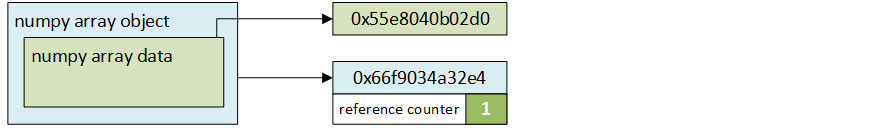
\includegraphics[width=0.99\textwidth]{img/array_creation_deletion_a}
        \caption{The NumPy array is created in Python. Note that the NumPy 
        object and the data it contains are represented by two separate memory addresses.}
        \label{fig:array_creation_deletion_a}
    \end{subfigure}
    \begin{subfigure}{0.9\textwidth}
        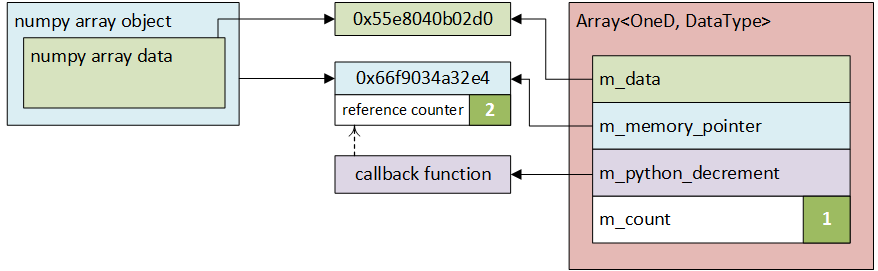
\includegraphics[width=0.99\textwidth]{img/array_creation_deletion_b}
        \caption{The C++ array is created through the converter method: its attributes 
        point to the appropriate memory addresses and the reference counter of the 
        memory address of NumPy array object is incremented.}
        \label{fig:array_creation_deletion_b}
    \end{subfigure}
    \begin{subfigure}{0.9\textwidth}
        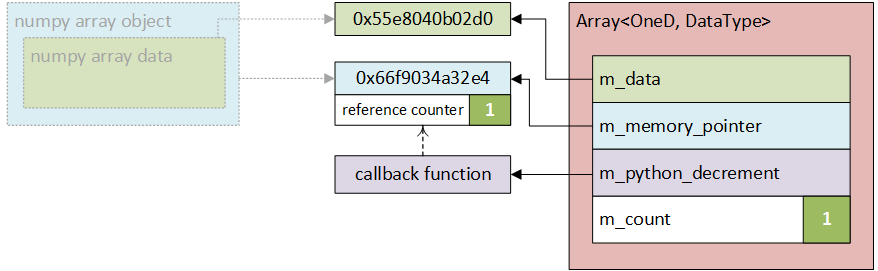
\includegraphics[width=0.99\textwidth]{img/array_creation_deletion_c}
        \caption{If the NumPy object is deleted first, the reference counter is 
        decremented, but the data still exists in memory.}
        \label{fig:array_creation_deletion_c}
    \end{subfigure}
    \begin{subfigure}{0.9\textwidth}
        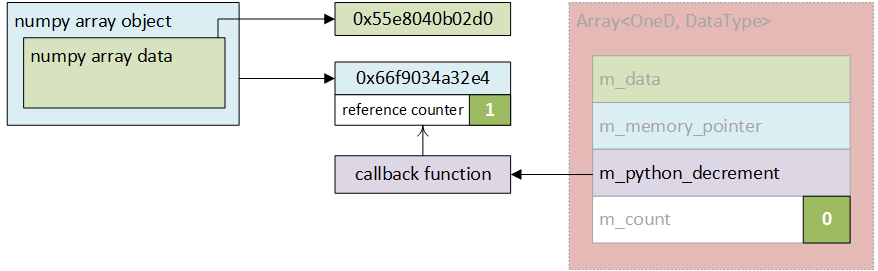
\includegraphics[width=0.99\textwidth]{img/array_creation_deletion_d}
        \caption{If the C++ array is deleted first, the callback function decrements 
        the reference counter of the NumPy object but the data still exists in memory.}
        \label{fig:array_creation_deletion_d}
    \end{subfigure}
    \caption{Diagram showing the process of creation and deletion of arrays. Reference 
    counters shown in green.}
    \label{fig:array_creation_deletion}
\end{figure}

\clearpage

\begin{figure}[h!]
    \centering
    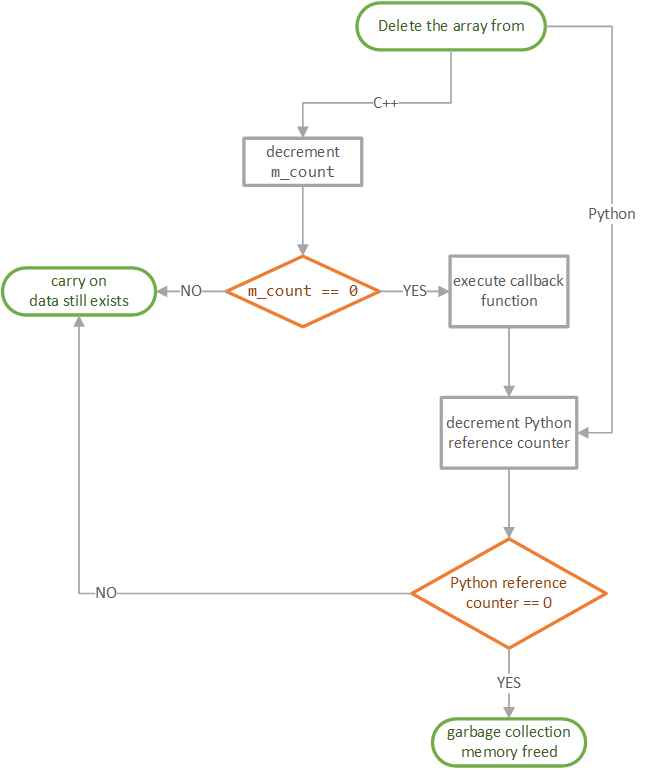
\includegraphics{img/deletion_flowchart}
    \caption{Flowchart describing the procedure for array deletion from either side of 
    the code.}
    \label{fig:array_deletion}
\end{figure}

\clearpage

\begin{lstlisting}[caption={Converter method for converting the Python NumPy arrays into C++ arrays.}, label={lst:python_to_c}, language=C++]
static void construct(
        PyObject *objPtr,
        py::converter::rvalue_from_python_stage1_data* data)
    {
        // Extract data from the PyObject.
        // This has to be a _borrowed_ reference, otherwise at the end of this
        // scope it seems memory gets deallocated
        py::object obj((py::handle<>(py::borrowed(objPtr))));
        np::ndarray array = py::extract<np::ndarray>(obj);
        
        // Get pointer to the memory into which the C++ type will be constructed
        void *storage = (
            (py::converter::rvalue_from_python_storage<Array<OneD, T> >*)data)
            ->storage.bytes;
        data->convertible = storage;
        
        // Grab the address of PyObject for C++ to use.
        void *memory_pointer = objPtr;
        
        // Remedies issues with using const datatypes.
        using nonconst_t = typename std::remove_const<T>::type;
        
        // Construct OneD array from numpy array.        
        new (storage) Array<OneD, T>(array.shape(0), // array size
            (nonconst_t *)array.get_data(), // pointer to the data readable by C++
            memory_pointer, // memory address of the PyObject
            &decrement); // pointer to the callback decrement function
        // Increment the Python reference counter.
        Py_XINCREF(objPtr);
    }
\end{lstlisting}

\subsubsection{Testing}

As the process of converting arrays from Python to C++ required making direct calls to 
C API and relying on custom-written methods, more detailed testing was deemed necessary. 
In order to thoroughly check if the conversion works as expected, three tests were 
conducted to determine whether the array is:

\begin{enumerate}
\item referenced (not copied) between the C++ program and the Python wrapper,
\item accessible to C++ program after being deleted in Python code,
\item accessible in Python script after being deleted from C++ objects.
\end{enumerate}

Python files containing test scripts are currently located in 
\path{library\Demos\Python\tests}. They should be converted into unit tests 
that should be run when Python components are built.
